\documentclass{acmtog}



\acmVolume{VV}
\acmNumber{N}
\acmYear{YYYY}
\acmMonth{Month}
\acmArticleNum{XXX}  
\acmdoi{10.1145/XXXXXXX.YYYYYYY}

%\acmVolume{28}
%\acmNumber{4}
%\acmYear{2010}
%\acmMonth{December}
%\acmArticleNum{106}  
%\acmdoi{10.1145/1559755.1559763}

\usepackage{subfig}
\usepackage{verbatim}
\usepackage{enumerate}

\usepackage{courier}

\usepackage{color}
\usepackage{xcolor}
\usepackage{listings}


 \lstset{
         basicstyle=\footnotesize\ttfamily, % Standardschrift
         %numbers=left,               % Ort der Zeilennummern
         numberstyle=\tiny,          % Stil der Zeilennummern
         %stepnumber=2,               % Abstand zwischen den Zeilennummern
         numbersep=5pt,              % Abstand der Nummern zum Text
         tabsize=2,                  % Groesse von Tabs
         extendedchars=true,         %
         breaklines=true,            % Zeilen werden Umgebrochen
         keywordstyle=\color{red},
    		frame=b,         
 %        keywordstyle=[1]\textbf,    % Stil der Keywords
 %        keywordstyle=[2]\textbf,    %
 %        keywordstyle=[3]\textbf,    %
 %        keywordstyle=[4]\textbf,   \sqrt{\sqrt{}} %
         stringstyle=\color{white}\ttfamily, % Farbe der String
         showspaces=false,           % Leerzeichen anzeigen ?
         showtabs=false,             % Tabs anzeigen ?
         xleftmargin=17pt,
         framexleftmargin=17pt,
         framexrightmargin=5pt,
         framexbottommargin=4pt,
         %backgroundcolor=\color{lightgray},
         showstringspaces=false      % Leerzeichen in Strings anzeigen ?        
 }
 \lstloadlanguages{% Check Dokumentation for further languages ...
         %[Visual]Basic
         %Pascal
         %C
         %C++
         %XML
         %HTML
         Java
 }

\usepackage{caption}
\DeclareCaptionFont{white}{\color{white}}
%\DeclareCaptionFormat{listing}{\colorbox{gray}{\parbox{\textwidth}{#1#2#3}}}
\DeclareCaptionFormat{listing}{\colorbox{gray}{\parbox{0.45\textwidth}{#1#2#3}}}
\captionsetup[lstlisting]{format=listing,labelfont=white,textfont=white}


\begin{document}
%\large

%\markboth{V. F. Pamplona et al.}{Photorealistic Models for Pupil Light Reflex and Iridal Pattern Deformation}

\title{Stable Fluids Paper Review and Demo Implementation} % title

\author{Jonathan Frawley
\affil{University of Dublin, Trinity College}
Original Paper by:\\
Jos Stam
\affil{Ulm University, Germany}
}

%\category{I.3.7}{Computer Graphics}{Three-Dimensional Graphics and Realism}[Photorealistic Rendering]
%\category{I.3.5}{Computer Graphics}{Computational Geometry and Object Modeling}[Physically based modeling]

\terms{Global Illumination, ray tracing}

\keywords{Ray tracing, photorealism}

%\acmformat{Pamplona, V. F., Oliveira, M. M., and Baranoski, G. V. G. 2009. Photorealistic models for pupil light
%reflex and iridal pattern deformation.  {ACM Trans. Graph.} 28, 4, Article 106 (August 2009), 11 pages.\newline  DOI $=$
%10.1145/1559755.1559763\newline http://doi.acm.org/10.1145/1559755.1559763}

\maketitle

\begin{abstract} 
The paper reviewed presents a simulator capable of creating fluid-like behaviour in a real-time fashion.
An implementation of the paper was created in the Processing programming language which simulates fluids in the same manner as is done in the paper.
\end{abstract}

\section{Introduction}
Simulating fluids is an important problem in computer graphics. 
Physical models of fluids allow for very convincing simulations to be created.
It was thought that simulating the physical models of fluids was too complex for real time applications.
The solver presented by Stam~\cite{DBLP:conf/siggraph/Stam99a} however allows for the stable physical simulation of fluids in real time.
The stability of the model is integral to its ability to be simulated in real-time, as previous techniques typically used unstable methods to solve the equations governing a fluid.
This stability allows the user to take larger time steps and achieve faster simulations without compromising the stability of the system.

The solver presented uses the \emph{Navier-Stokes} equations to simulate fluid flow.
Fluid solvers in computer graphics typically weight real-time interactivity higher than strict physical accuracy, which engineering-type applications would be interested in.
Most computer graphics applications tended to use simple primitives such as particles~\cite{Reeves83particlesystems}.
The complexity of such simulations was increased with the introduction of random turbulences~\cite{Chen97real-timefluid}.
These exhibit rotational motion and are mass conserving. 
However flows built up from a superposition of flow primitives will not react dynamically to forces applied by the user in real-time as we desire.

Models which use the \emph{Navier-Stokes} equations first were implemented in 2-dimensions.
Gamito et al. used a vortex method with a poisson solver to create two-dimensional animations of fluids~\cite{Gamito95two-dimensionalsimulation}.
Chen et al. later animated water surfacts from the pressure term given by the \emph{Navier-Stokes} equations~\cite{Chen97real-timefluid}.
These methods of solving Navier-Stokes is both unstable and limited to two dimensions. 
Many effects arise from using the full \emph{Navier-Stokes} equations such as swirling motion and flows past objects.
Explicit solvers for the \emph{Navier-Stokes} equations were created by Foster and Metaxas~\cite{Foster97modelingthe} but have the disadvantage of being unstable for large time steps.
This instability sets limits on the speed and interactivity of these simulations, where a user might have to restart the simulation if it ``blows up'' unexpectedly.

The method created by Stam is both stable and uses the three dimensional form of the \emph{Navier-Stokes} equations.
It is able to use timesteps which are much larger than that of Foster and Metaxas and thus is able to achieve real-time speed.
The method uses Lagrangian and implicit methods to solve the \emph{Navier-Stokes} equations over the Eulerian techniques previously used.
The model presented is not accurate enough for engineering applications as it suffers from ``numerical dissipation'' but it is ideal for real time applications where the user is repeatedly applying new forces.

\section{Background}
This section will describe the \emph{Navier-Stokes} equations and the implementation of the stable solver.
A fluid is described by a velocity field $ u $ and a pressure field $ p $. 
The spatial coordinate will be denoted by $ x $ which will be a 2D or 3D vector, depending on the dimensionality of the implementation.
The demo implemented uses 2D vectors for all quantities but it can easily be generalised to 3 dimensions.
We assume that the velocity and the pressure are known at time $ t=0 $ and the evolution of these quantities over time is given by the \emph{Navier-Stokes} equations:
\begin{equation}
  \nabla \cdot u = 0
\end{equation}
\begin{equation}
  \label{eq2}
  \frac{\partial u}{\partial t} = -(u \cdot \nabla)u - \frac{1}{\rho} \nabla p + v \nabla^{2}u + f
\end{equation}
where v is the kinematic viscosity of the fluid, $\rho$ is its density, $f$ is an external force, $\nabla$ is the vector of spatial partial derivatives(e.g in two dimensions $\nabla = (\frac{\partial}{\partial x}, \frac{\partial}{\partial y}$).
These equations assume that mass and momentum are conserved.
Boundary conditions will be used to supplement these equations.
We consider 2 boundary conditions, 1 fixed where walls prevent the fluid from escaping, and 1 periodic, where the fluid wraps around.

The implementation of the fluid solver by Stam uses a modification on the above equation, using a mathematical result known as the \emph{Helmholtz-Hodge Decomposition} which states that any vector field $w$ can be uniquely decomposed into the form:
\begin{equation}
w = u + \nabla q
\end{equation}
where $u$ has zero divergence. This allows us to define an operator $P$ which projects any vector field $w$ onto its divergence free part $u = Pw$:
\begin{equation}
\label{eq4}
\nabla \cdot w = \nabla^{2}q
\end{equation}
A solution to this equation is used to compute the projection $u$:
\begin{equation}
u = P w = w - \nabla q
\end{equation}
which we can apply to both sides of Eq.~\ref{eq2} to obtain a single equation for velocity:
\begin{equation}
  \label{eq5}
  \frac{\partial u}{\partial t} = P(-(u \cdot \nabla)u + v \nabla^{2}u + f)
\end{equation}
which is the fundamental equation used to develop the stable fluid solver.

Eq.~\ref{eq5} is solved from the initial state $u_0 = u(x,0)$ by iteratively progressing time by a time step $\Delta t$.
At every step we have the solution to the equation at time $t$ and wish to compute it at the next time interval $t + \Delta t$.
The equation is solved in 4 steps:
\begin{enumerate}
\item $w_{0} \to w_{1}$ : Add force
\item $w_1 \to w_2$ : Advect
\item $w_2 \to w_3$ : Diffuse
\item $w_3 \to w_4$ : Project
\end{enumerate}
Where the solution is given by the last velocity field, $w_4$.
The first term is the addition of the external force which is defined as:
\begin{equation}
w_1(x)=w_0(x) + \Delta t f(x,t)
\end{equation}

The next term accounts for the effects of advection, also known as convection.
This accounts for the subexpression $ -(u \cdot \nabla)u $ from Eq.~\ref{eq5}.
The method used to solve this part of the equation is known as the \emph{method of characteristics} and is detailed by Pironneau~\cite{pironneau2000method} and is also explained by Stam as an appendix~\cite{DBLP:conf/siggraph/Stam99a}.
The core concept is that instead of working forwards in time, we try to work backwards.
In order to obtain the velocity of the point $x$ at the new time $t + \Delta t$ we backtrace the point $x$ through the velocity field $w_1$ over a time $\Delta t$. 
This defines a path $p(x, s)$ which corresponds to a partial streamline through the velocity field.
The new velocity at the point $x$ is then set to the velocity that the particle had $\Delta t$ ago:
\begin{equation}
w_2(x) = w_1(p(x, - \Delta t))
\end{equation}

The third term accounts for the effect of viscosity and is equivalent to a diffusion equation:
\begin{equation}
\frac{\partial w_2}{\partial t} = v \nabla^2 w_2
\end{equation}
which is solved using an implicit method:
\begin{equation}
(I-v \Delta t \nabla^2) w_3(x) = w_2(x)
\end{equation}

The fourth step involves the projection step which makes the resulting field divergence free.
This involves resolving Eq.~\ref{eq4}:
\begin{equation}
\nabla^2q = \nabla \cdot w_3 , w_4 = w_3 - \nabla q
\end{equation}
This is solved again using the method of characteristics.

The algorithm described in this section has performance $O(N)$ where $N$ is the size of the input grid.
The above description uses the method of characteristics to solve the equations.
We will now focus on the implementation of a more modern fluid solver which uses Gauss-Seidel relaxation as an iterative solver instead.

\section{Demo Implementation}
The implementation of the fluid solver demo created for this project is based primarily on Stam's later work on fluid dynamics for games~\cite{stam2003real}.
This paper gives a more practical implementation of the solver described by Stam.
This uses a concept known as smoke density, which can easily be visualised. 
This is a grid between zero and one, where zero indicates that no smoke is present and one indicates that it is consumed with smoke.
The demo uses this density function to visualise smoke in the scene. 

It was decided to focus on creating a 2D scene which used Stam's fluid equations to create smoke like effects.
The domain is limited to a square, as done by Stam~\cite{stam2003real}.
This square is of length $N+2$ as the extreme grid cells are used to either prevent smoke from leaving the box, or wrapping the smoke around in on itself and have to be treated specially.

\begin{figure}
  \caption{The 2D environment broken into an $(N+2) * (N+2)$ grid.}
  \centering
    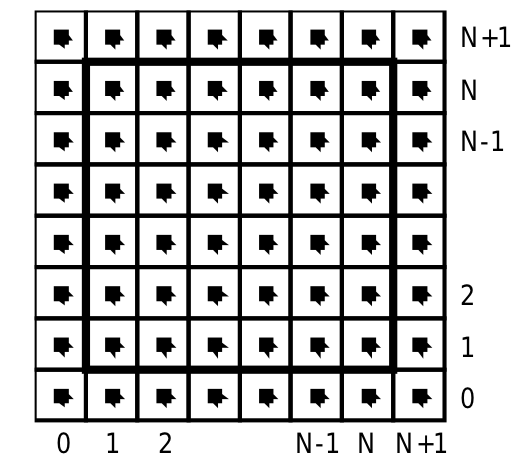
\includegraphics[width=0.5\textwidth]{images/grid}
\end{figure}

The velocity and the density at each grid cell is constant.
The velocity and densities are stored in 1D arrays for efficiency reasons.
The arrays are of length $size = (N+2) * (N+2)$ and array elements are accessed using the method in listing~\ref{ls1}.
\lstinputlisting[label=ls1,caption=Array index function, language=java]{code/ix.java}

The demo contains the environment within the 0.0 - 1.0 range on the x and y axes, so each grid cell has size $ h = 1 / N $.
The variable dt contains the fixed timestep between iterations.

\begin{figure*}
\centering
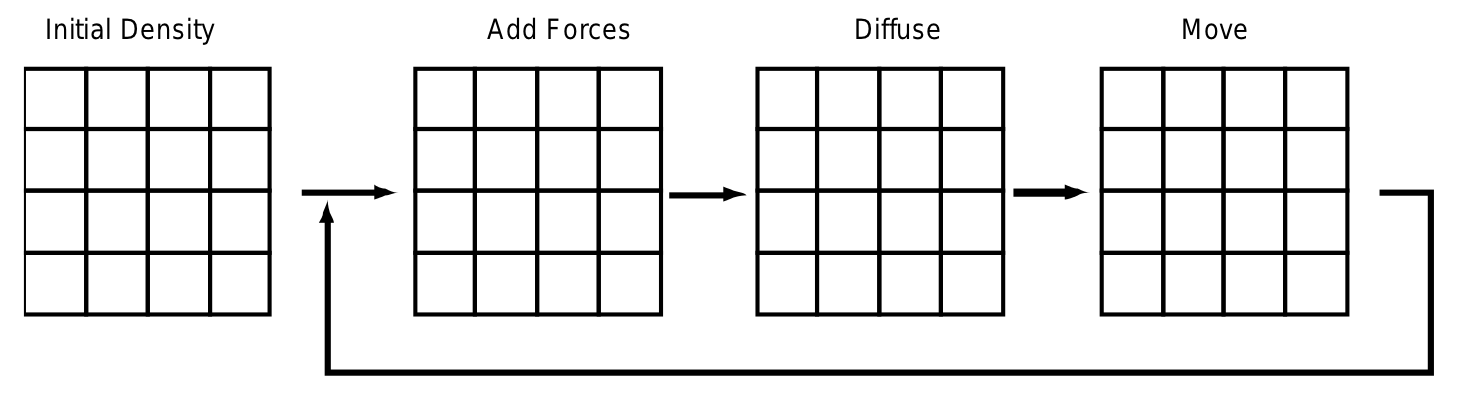
\includegraphics[width=1\textwidth]{images/density_solver}
  \caption{Structure of density solver, the three right hand terms are evaluated at each time step.}
\end{figure*}

The three right hand terms match up with the three terms on the right-hand side of the density Navier Stokes equation:
\begin{equation}
  \frac{\partial \rho}{\partial t} = -(u \cdot \nabla)\rho + \kappa \nabla^{2}\rho + S
\end{equation}

The theory for implementing the density solver is very similar to the velocity solver described previously.
The first term is simply the addition of sources of density based on the timestep, this allows users to add density dynamically.
\lstinputlisting[label=ls1,caption=Add Density source function, language=java]{code/source.java}

The second term represents the diffusion of density through the system which can be done by Gauss-Seidel relaxation.
This involves trying to extrapolate the densities which when we go back in time yield the current densities.
This has the same property as the method of characteristics in that it is stable.
\lstinputlisting[caption=Diffusion function, language=java]{code/diffuse.java}

The next stage of our density solver is the advection step which forces the density to follow a given velocity field.
We use a simple linear backtrace to determine the density which will follow the velocity field. 
This works by modelling the density as particles, and knowing that these particles will carry with them an amount of density which is retrieved by linear interpolating the density forwards in time based on the previous density values.
\lstinputlisting[caption=Advection step, language=java]{code/advect.java}

This is the density solver description in full.
Some of the functions have been modified for the demo for additional features as can be seen in the full source code.

We now turn our attention to the velocity solver, which reuses some of the functions from the density solver such as ``addSource'', ``diffuse'' and ``advect''.
It also adds in another function ``project'' which forces the velocity to be mass conserving. 
As described earlier, mass conserving fluids have the important property that they produce realistic swirly-like flows.
The routine uses a concept known as the Hodge decomposition~\cite{pirashvili2000hodge}.
This means that every velocity field is the sum of a mass conserving field and a gradient field.
To obtain an incompressible field we subtract the gradient field from our current velocities.
This involves computing the result of a Poisson equation which is done by Gauss-Seidel relaxation again.
The implementation is in the source code and will not be listed here for brevity.

When I had the initial implementation of the velocity and density solvers created as a demo in Processing, I decided to add some additional functionality.
For instance it is possible to add dynamic obstacles, toggle between visualising the velocity and density fields, and also visualising the density fields as a multicoloured gas to produce a flame-like effect.

\section{Conclusion}
Implementing this fluid solver has given me an appreciation for techniques for solving linear systems usch as Gauss-Seidel relaxation which I had not encountered before. 
The ease of implementation of these methods has made it easier to learn the concepts behind the solvers.
The papers I have read have been very practical and easily gave enough detail to implement my own version of the solver in Processing without looking at too many additional papers.
By implementing additional functionality beyond what was described in the paper, I have achieved a greater understanding of the system as a whole.

The results of interactive fluid simulations I do not believe have been fully taken advantage of in modern computer games.
This is surprising after having implemented this demo as I can not find a problem with simulating fluids in real-time.
The results look very natural and are relatively simple to implement.

The toughest part of the project was trying to figure out the best way to visualise the density information from the fluid solver. 
I came to a compromise and implemented 2 schemes, one which simply colours the pixel a shade of white with relative brightness to the amount of density present, and one which has a threshold which colours the pixel a reddish colour when its density is low and a more yellow-orange colour when its density rises. 
This gives a fire-like effect with very interesting results.
\begin{figure}
  \caption{Screenshot of demo in action with fire-like effect enabled}
  \centering
    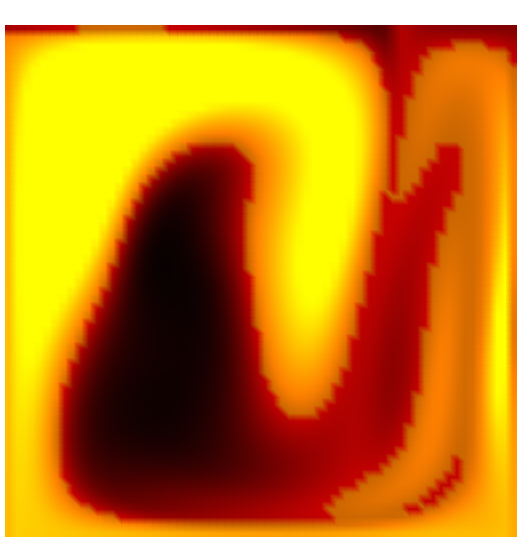
\includegraphics[width=0.3\textwidth]{images/demo}
\end{figure}

Implementing the demo gave me a great understanding of how things like velocity effect the simulation.
In the demo it is possible to toggle viewing the velocity on and off which greatly aided in my understanding of how the densities are propogated around the environment.

The fluid solver is very stable and I would recommend its use in 3D games.
It's big-oh complexity is known and is very acceptable, especially considering it is stable as other techniques for simulating fluids are not.


\bibliographystyle{acmtog}
\bibliography{main}

\received{December 2010}{December 2010}

\end{document}
